\documentclass[12pt,a5paper]{article}

\usepackage[T1]{fontenc} % font encoding, lubab õ tähte kasutada
\usepackage[utf8]{inputenc} % oleme siiski 21. sajandis, vajadusel on ka olemas utf8x
\usepackage{lmodern} % lmodern ja micrtype käivad käsikäes, teeb teksti ilusamaks
\usepackage{microtype}
\usepackage{tikz}
\usetikzlibrary{decorations.pathreplacing, positioning}
\usetikzlibrary{arrows,calc,decorations.markings,math,arrows.meta}

%\SIdecimalsign{,}
\usepackage{amsmath,amssymb} 
\usepackage{amsfonts}
\usepackage[estonian]{babel} % eesti keele poolitamisreeglid jpm
\usepackage[per = fraction, expproduct=cdot, decimalsymbol=comma]{siunitx} % http://www.bakoma-tex.com/doc/latex/siunitx/siunitx.pdf
\usepackage{graphicx} 
\usepackage{wrapfig}
\usepackage{epstopdf} %minul on vaja, et .eps pilte saada
\usepackage{float}

%paneme kõik mõõdud paika
\topmargin=-2.5cm \textheight=18cm \textwidth=12.77cm
\oddsidemargin=-1.5cm \evensidemargin=-1.5cm
\setlength{\parindent}{0pt} \setlength{\parskip}{6pt} \sloppy

\relpenalty=10000 \binoppenalty=10000 % Tekstisisestes valemites reavahetusi ärgu olgu


\pagestyle{empty} % ilma leheküljenumbrita

\newcommand{\numb}[1]{\vspace{5pt}\textbf{\large #1}}
\newcommand{\nimi}[1]{(\textsl{\small #1})}
\newcommand{\punktid}[1]{(\emph{#1~p.})}
\newcommand{\autor}[1]{\emph{ Autor: #1.}}
\newcounter{ylesanne}
\newcommand{\yl}[1]{\addtocounter{ylesanne}{1}\numb{\theylesanne.} \nimi{#1} \newblock{}}
\newcommand{\D}{\textrm{d}}

\tikzset{
	odot/.style={
		circle,
		inner sep=0pt,
		node contents={$\odot$},
		scale=2
	},
	otimes/.style={
		circle,
		inner sep=0pt,
		node contents={$\otimes$},
		scale=2
	},
	circ/.style={
		circle,
		draw,
		minimum size=3mm,
		inner sep=0
	},
	odot2/.style={
		circ,
		path picture={\fill circle[radius=1pt];}
	},
	otimes2/.style={
		circ,
		path picture={
			\draw (path picture bounding box.45) -- (path picture bounding box.225);
			\draw (path picture bounding box.135) -- (path picture bounding box.315);
		}
	}
}

\begin{document}

\begin{center}
\textbf{\large Eesti koolinoorte 31. füüsika lahtine võistlus} \vspace{3pt}

\emph{21. november 2020. a. Vanema rühma ülesannete lahendused}
\end{center}



\yl{PUDEL}
Olgu algne vee ruumala pudelis $V_0$. Selleks, et ära joodud vee ruumala maksimeerida, peaks ilmselt lõpus pudelit ainult õhk täitma. Vastasel korral on võimalik algset vee ruumala vähendada ning suurema õhu osakaalu arvelt rohkem vett ära juua.

Pudelist joomine on isotermiline protsess. Seega,
\[
p_0 (V-V_0)=(p_0-\Delta p)V.
\]
Siit avaldades $V_0$ saame, et
\[
V_0=\frac{\Delta P}{p_0} V = \num{0.25} V.
\]
\punktid{6} \autor{Kaarel Kivisalu}


\yl{RUUT FOOKUSES}
\begin{figure}[H]
	\centering
	\resizebox{\linewidth}{!}{%
		\begin{tikzpicture}[scale=1]
			\filldraw[black] (-2,0) circle (2pt) node[anchor=south west] {$F$};
			\filldraw[black] (2,0) circle (2pt) node[anchor=south] {$F$};
			\filldraw[black] (0,0) circle (2pt) node[anchor=south west] {$O$};
			\filldraw[black] (-1,1) circle (2pt) node[anchor=south] {$A$};
			\filldraw[black] (-1,-1) circle (2pt) node[anchor=north] {$B$};
			\filldraw[black] (-3,-1) circle (2pt) node[anchor=north] {$C$};
			\filldraw[black] (-3,1) circle (2pt) node[anchor=south] {$D$};
			\draw[gray] [dashed,-] (-5,0) -- (10,0);
			\draw[black, line width=1.5pt] (-1,1) -- (-1,-1);
			\draw[black, line width=1.5pt] (-1,-1) -- (-3,-1);
			\draw[black, line width=1.5pt] (-3,-1) -- (-3,1);
			\draw[black, line width=1.5pt] (-3,1) -- (-1,1);
			
			\draw[line width=2pt,>=stealth, <->] (0,-2) -- (0,2);
			
			\draw [dotted] (-1,1) -- (0,1);
			\draw [dotted] (-1,-1) -- (0,-1);
			\draw [dotted] (-5,-3.5) -- (10,4);
			\draw [dotted] (-5,3.5) -- (10,-4);
			
			\draw [dotted](0,0) -- (-5,5);
			\draw [dotted](0,0) -- (-5,-5);
			\draw [dotted](-3,-1) -- (10, 3.3333);
			\draw [dotted](-3,1) -- (10,-3.3333);
			
			\filldraw[black] (-2,2) circle (2pt) node[anchor=south] {$A'$};
			\filldraw[black] (-2,-2) circle (2pt) node[anchor=north] {$B'$};
			\filldraw[black] (6,2) circle (2pt) node[anchor=north west] {$C'$};
			\filldraw[black] (6,-2) circle (2pt) node[anchor=south west] {$D'$};
			
			\draw[black,line width=1pt] (-2, 2) -- (-2,  -2);
			\draw[black,line width=1pt] (-2, 2) -- (-5, 3.5);
			\draw[black,line width=1pt] (-2,-2) -- (-5,-3.5);
			\draw[black,line width=1pt] ( 6, 2) -- ( 6,  -2);
			\draw[black,line width=1pt] ( 6, 2) -- ( 9,  3.5);
			\draw[black,line width=1pt] ( 6,-2) -- ( 9, -3.5);
			\draw[black,line width=1pt,dashed] ( 9,-3.5) -- (10, -4);
			\draw[black,line width=1pt,dashed] ( 9, 3.5) -- (10,  4);
			\draw[black,line width=1pt,dashed] (-5,-3.5) -- (-6, -4);
			\draw[black,line width=1pt,dashed] (-5, 3.5) -- (-6,  4);
			
			\filldraw[black] (-2.6,1) circle (2pt) node[anchor=south] {$K$};
			\filldraw[black] (-1.4,1) circle (2pt) node[anchor=south] {$L$};
			\filldraw[black] (-4.667,3.333) circle (2pt) node[anchor=south] {$L'$};
			\filldraw[black] (8.667,-3.333) circle (2pt) node[anchor=south] {$K'$};
			\draw [dotted](0,0) -- (-4.667,3.333);
			\draw [dotted](-2.6,1) -- (8.667,-3.333);
		\end{tikzpicture}
	}%
\end{figure}
Leiame punktide $A, B, C$ ja $D$ kujutised $A', B', C'$ ja $D'$ läätses eraldi. Ühendame vertikaalsed küljed $A'B'$ ja $C'D'$. Märkame, et punktid $A'$ ja $B'$ on teisel pool läätse kui punktid $C'$ ja $D'$. Seega ei ole lõigu $AD$ kujutis lõik $A'D$. Valime küljel $AD$ abipunktid $K$ ja $L$, mis asuks vastavalt vasakul ja paremal pool fookusest. Seega on külje $AD$ fookusest paremal oleva osa kujutis sirgel $A'L'$ ja fookusest vasakul oleva osa kujutis sirgel $D'K'$. Kuna mistahes $L$ ja $K$ puhul on need fookusele lähemal kui $A$ ja $D$, siis on ka lõigust $AD$ iga punkti kujutis läätsest kaugemal, kui $A'$ ja $D'$.
Analoogselt leiame ka $BC$ kujutise.
\punktid{8} \autor{Hannes Kuslap}


\yl{U-KLAAS}
Esmalt teeme selgeks, milline peaks olema kõverusraadius, et esimese peegelduse jaoks oleks kogu valgusvihu ulatuses langemisnurk suurem kui kriitiline nurk. On ilmne, et kõige väiksem on langemisnurk valgusvihu kõige sisemise (joonisel parempoolse) kiire jaoks. Joonistame kiire käigu kriitilise nurga korral.

\begin{center}
	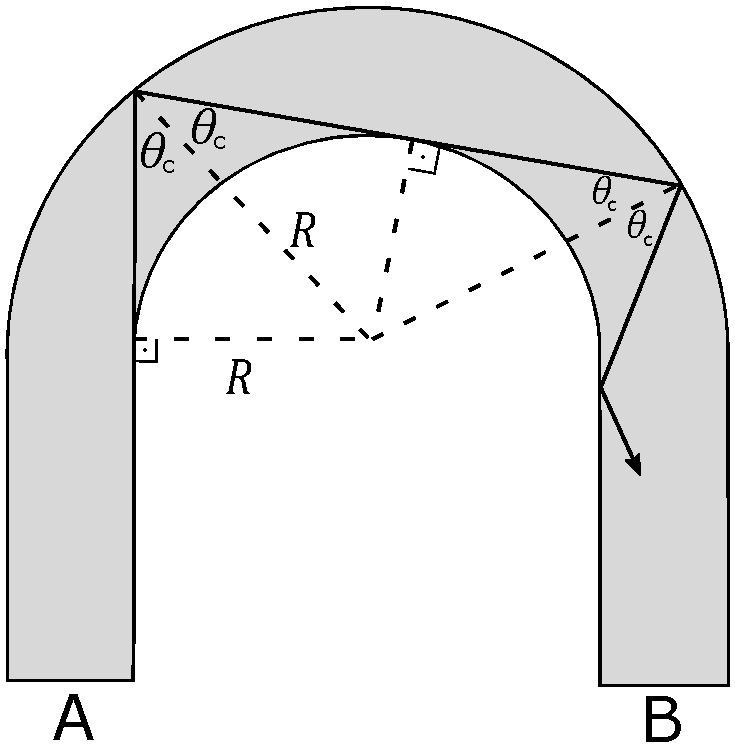
\includegraphics[width=0.6\textwidth]{uklaas_lah.pdf} 
\end{center}

Snelli seadusest täieliku sisepeegeldumise jaoks
$\sin\theta_c = {1}/{n}$, jooniselt saame, et $\sin\theta_c=R/(R+d)$. Seega
$$\frac{1}{n}=\frac{R}{R+d}\Rightarrow R = \frac{\SI{3}{\cm}}{1.5-1}=\SI{6}{cm}.$$
Paneme tähele, et peegeldunud kiir puutub sümmeetria tõttu klaasitüki sisekülge ning peegeldub välisküljelt sama nurga all kui esimene kord. Sama protsess kordub, kuni klaasi kõver osa läheb üle sirgeks. Sellisel juhul on langemisnurk suurem kui enne ning toimub kindlasti peegeldumine ja lõpuks on tagatud, et valgusvihk väljub läbi tahu B. Järelikult ongi ainsaks tingimuseks esimesest peegeldusest saadu, mis annab $R\geq\SI{6}{\cm}$.
\punktid{8} \autor{Hans Daniel Kaimre}


\yl{NOOVA}
Vaatleme jäänuki liikumist aja $t$ jooksul, selle aja jooksul liigub jäänuk vahemaa $vt$. Näeme, et ristisihis liigub jäänuk vahemaa $vt \sin \theta$, seega kasutades väikeste nurkade lähendusi, on Jarli poolt mõõdetav nurk nende kahe positsiooni vahel $\alpha = vt\sin\theta/D$ ja näiv vahemaa, mille jäänuk nende hetkede vahel läbib on
\begin{equation*}
	x' = \alpha D = vt\sin\theta.
\end{equation*}

\begin{figure}[h]
\centering
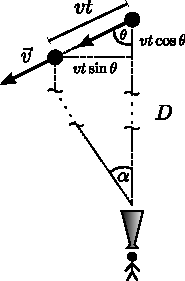
\includegraphics[width=0.25\linewidth]{noova_lah_joon}
\end{figure}

Küll aga tuleb arvestada ka sellega, et jäänuk liigub selle aja jooksul $vt \cos\theta$ vaatesihis Jarlile lähemale, mistõttu teepikkus, mille valgus peab Jarlini jõudmiseks läbima, lüheneb ja seega näiv aeg kahe hetke vahel $t'$ ei ole võrdne tegeliku ajaga $t$. Kuna esimesel hetkel on jäänuki kaugus Jarlist $D$ ning teisel juhul $D-vt\cos\theta$ (kasutades lähendust, et $D$ on väga suur), siis näiv aeg kahe hetke vahel on
\begin{equation*}
t' = t_2 - t_1 = \left(t + \frac{D-vt\cos\theta}{c}\right) - \frac{D}{c} = t\left(1 - \frac{v\cos\theta}{c}\right).
\end{equation*}

Seetõttu Jarli poolt mõõdetav näiv kiirus on
\begin{equation*}
v' = \frac{x'}{t'} = \frac{v \sin \theta}{1- \frac{v}{c}\cos\theta}.
\end{equation*}

Näeme, et näiv kiirus võib olla tõesti suurem kui $c$. Näiteks kui $\theta = 45^\circ$ ja $v = \frac{7}{5\sqrt 2}c$ (mis on väiksem kui $c$), siis
\begin{equation*}
v' = \frac{\frac{7}{5\sqrt 2} c \cdot \frac{1}{\sqrt 2}}{1- \frac{7}{5\sqrt 2} \cdot \frac{1}{\sqrt 2}} = \frac{7}{3} c > c.
\end{equation*}

\textit{Märkus.} Selline nähtust, kus näiv kiirus on valguse kiirusest suurem (ingl. k. \textit{superluminal motion}), on märgatud mitmete astronoomiliste objektide korral. Üks suuremaid näivaid kiirusi on mõõdetud kvasarijoa korral, mille näivaks kiiruseks mõõdeti $\num{9.6}c$.
\punktid{10} \autor{Richard Luhtaru}


\yl{SOLENOID JA KONTUUR}
Solenoidi sees on magnetiline induktsioon $B = \mu_0 nI$. Vastavalt Faraday induktsiooniseadusele on kontuuris tekkiv induktsiooni elektromotoorjõud absoluutväärtuselt võrdne kontuuri läbiva magnetvoo $\Phi=BS$ muutumise kiirusega:
\[
\epsilon=\frac{\Delta \Phi}{\Delta t}=S\frac{\Delta B}{\Delta t}=\mu_0 n S \frac{\Delta I_s}{\Delta t},
\]
kus $S=\pi r^2$ on solenoidi ristlõikepindala ja $r$ on ristlõike raadius. Selgitava märkusena olgu öeldud, et elektromotoorjõu vahetu tekitaja on solenoidi ümbritsev pööriselektriväli, mis on tingitud muutuvast magnetväljast solenoidi sees. Elektromotoorjõu tõttu tekib kontuuris vool $I=\epsilon/R =\epsilon S_0/(\rho l)$, kus $l$ on kontuuri pikus.
Tekkiv vool on maksimaalne, kui voolu $I_s$ muutumise kiirus $\Delta I_s/\Delta t$ on absoluutväärtuselt suurim. Funktsiooni $I_s(t)$ graafikult näeme, et see juhtub ajahetkel $t\approx \SI{0,9}{s}$. Vahemikus 
$t=\SI{0.85}{s} \ldots \SI{0.95}{s}$ on $I_s(t)$ graafik ligikaudu sirge ja seega $|\Delta I_s/\Delta t|_{max} \approx (\num{0,6}-\num{0,1})/(\num{0,95}-\num{0,85})=\SI{5}{mA/s}$. Teiselt jooniselt saame solenoidi raadiuse $r=\SI{2}{cm}$ ja kontuuri pikkuse $l=\SI{40}{cm}$. Voolutugevuse maksimaalne väärtus kontuuris on seega
\[
I_{\mathrm{max}}=\frac{\mu_0 \pi r^2 n S_0 }{\rho l}\left|\frac{\Delta I_s}{\Delta t}\right|_{\mathrm{max}}\approx \SI{1,5}{\mu A}.
\]
\punktid{10} \autor{Päivo Simson}


\yl{KONDENSAATORID}
Peale lüliti avamist pole punkt $A$ enam ülejäänud skeemiga juhtmete kaudu ühendatud. Kuna laengud ei saa läbi õhu hüpata (pinged on läbilöögitugevusest palju väiksemad), kehtib skeemi $A$ poolses osas laengu jäävus.

Alguses on $A$ ja $B$ vaheline pinge $V_1 = \mathcal E$. Punkti $A$ suhtes on $C_1$ ja $C_2$ pinged vastavalt \SI{0}{V} ja $\mathcal E$. Järelikult on $C_1$ ja $C_2$ sisemiste plaatide kogulaeng $q_\mathrm{tot} = 0 + C_2\mathcal E = C_2\mathcal E$.

Olgu punktide $A$ ja $B$ vaheline pinge peale lüliti avamist $V_2$. $C_1$ ja $C_2$ pinged punkti $A$ suhtes on siis $V_2 - \mathcal E$ ning $V_2$ ja sisemiste plaatide kogulaeng on $q_\mathrm{tot} = C_1(V_2 - \mathcal E) + C_2V_2$. Kokkuvõttes saame
\[
q_\mathrm{tot} = C_2\mathcal E = C_1(V_2 - \mathcal E) + C_2V_2,
\]
millest $V_2=\mathcal E$. Näeme, et pinge punktide $A$ ja $B$ vahel ei muutu.
\punktid{10} \autor{Taavet Kalda}


\yl{POOLSILINDER BASSEINIS}
Vaatleme poolsilindrit ning selle kohal olevat veesammast ühtse kehana. Me saame seda teha, sest süsteem on tasakaalus ning vesi on paigal.
Paneme esmalt kirja jõudude tasakaalu vertikaalsihis.
Vertikaalsihis mõjub raskusjõud ning poolsilindri ja põranda vaheline toereaktsioon $N$.

Poolsilindri kohal oleva veesamba ruumala on
\begin{equation*}
	V_{\mathrm{vesi}}=l r^2-\pi \frac{r^2 l}{4}=l r^2\left(1-\frac{\pi}{4}\right).
\end{equation*}
Seega, vertikaalne jõudude tasakaal avaldub kujul
\begin{equation*}
	N=g(\rho V_{\mathrm{vesi}} + m) = g\left(\rho l r^2\left(1-\frac{\pi}{4}\right) + m\right).
\end{equation*}
Teades reaktsioonijõudu $N$ on lihtne leida hõõrdejõud poolsilindri ja põhja vahel:
\begin{equation*}
	F_{\mu}=\mu N= \mu g \left(\rho l r^2\left(1-\frac{\pi}{4}\right) + m\right).
\end{equation*} 
Horisontaalsuunas tasakaalustab hõõrdejõudu vee horisontaalsuunaline rõhumisjõud $F_{\mathrm{vedelik}}$. Poolsilindri ja selle kohal olevale veesamba süsteemile mõjub keskmiselt rõhk $p = \rho gr/2$, kusjuures kontaktpindala on $S = lr$. Järelikult on horisontaalsuunaline jõud
\begin{equation*}
	F_{\mathrm{vedelik}}=\frac{\rho g r}{2}r l=\frac{\rho g l r^2}{2} F_{\mu}.
\end{equation*}
Kombineerides mõlemad avaldised $F_\mu$ jaoks, saame
\begin{equation*}
	\mu_0=\frac{\rho l r^2}{2(\rho l r^2(1-\frac{\pi}{4})+m}.
\end{equation*}
\punktid{10} \autor{Krister Kasemaa}


\yl{TERMOKAAMERA}
Kuivõrd plaat on väike, siis tema kiirgus ei mõjuta märkimisväärselt toa üldist soojuskiirguse fooni, mis vastab absoluutselt musta keha soojuskiirguse energiavoo tihedusele $\sigma T^4$. Seetõttu ``näeb'' soojuskaamera vaskplaadilt lähtuvat kahte kiirguskomponenti: 97\% kiirgusest moodustab plaadile langenud ja sellelt peegeldunud foonikiirgust ning 3\% moodustab plaadi enda soojuskiirgus. Seega saame seose $\sigma T_2^4= \num{0.97}\sigma T_0^4+\num{0.03}\sigma T_1^4$, millest 
$$T_1=[(T_2^4-\num{0.97}T_0^4)/\num{0.03}]^{1/4}\approx \SI {345}K\approx \SI{72}\celsius.$$
\punktid{12} \autor{Jaan Kalda}


\yl{SUVI}
Maa liigub mööda ellipsit, kusjuures Päike asub selle pikemal sümmeetriateljel (pikemal poolteljel). Olgu Päike punktis $F$ ning orbiidi punktid, kus algavad suvi ja talv, vastavalt $S$ ja $T$, sest ülesande eeldusest teame, et Maa on Päikesele kõige lähemal suvisel pööripäeval. Tähistame suve ja talve lõpu punkti orbiidil vastavalt $S'$ ja $T'$. Suvi lõppeb, kui Maa telg on risti Päikest ja Maad ühendava lõiguga ning kuna telje suund aasta jooksul ei muutu, siis $\angle SFS' = \ang{90}$. Kepleri 2. seaduse järgi on suve ja talve pikkused võrdeliselt vastavalt kujundite $FSS'$ ja $FTT'$ pindaladega. Kõige mugavam on seda võrrelda ellipsi kogupindalaga, $S_0$. Sellisel juhul on suve pikkus $T_S = T_\oplus S_{FSS'}/S_0 $ ning talve pikkus $T_T = T_\oplus S_{FTT'}/S_0$, kus $T_\oplus = T =\SI{365.26}{päeva}$ on Maa orbitaalperiood.	

Ellipsi pindala on veel leitav, aga kujundite $FSS'$ ja $FTT'$ pindalade arvutamine on väga keeruline. Aitab tähelepanek, et ellips on väljavenitatud ring. Kuna $T_S$ ja $T_T$ sõltuvad vastavate kujundite pindalade suhtest kogupindalaga, võime ellipsit ühes suunas välja venitada ilma et see otsitavaid suhteid muudaks. Seega võime mugavuse pärast ellipsi ringiks venitada, vaata joonist. Joonisel kujutatud pindalad 1 ja 2 suhtuvad ellipsisse ning ringi samasuguste suhetega.

\begin{figure}[H]
	\centering
	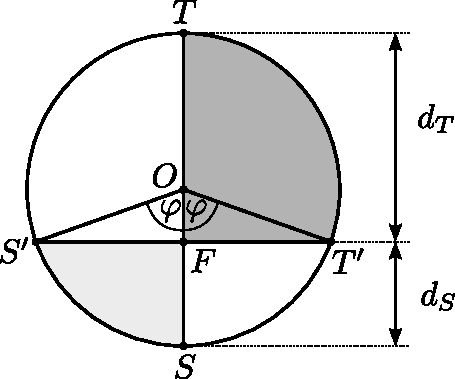
\includegraphics[width=0.4\linewidth]{suvi-joonis-2.pdf}
\end{figure}

Edaspidi arvutame kõik pindalad ringiks venitatud ellipsi peal (vaata teist joonist), olgu ringi keskpunkt $O$.


Olgu Maa kaugused Päikesest suvisel ja talvisel pööripäeval vastavalt $d_S$ ja $d_T$. Vaatleme nüüd sfääre raadiustega $d_S$ ja $d_T$, mille keskpunktides on päike. Kuna sfääri pindala on proportsionaalne selle raadiuse ruuduga ning summaarne kiirgusenergia, mis jõuab kaugusele $d_T$ on sama, mis jõuab kaugusele $d_S$, siis järelikult on Päikese heledus pöördvõrdeline kauguse ruuduga. Seega saame, et
\[
\left(\frac{d_T}{d_S}\right)^2 = k^2 = \num{1.3},
\]
kus $k = \sqrt{\num{1.3}}$ on konstant valemite mugavamaks kirjapanekuks. Niisiis, $d_T = kd_S$.

\begin{figure}[H]
	\centering
	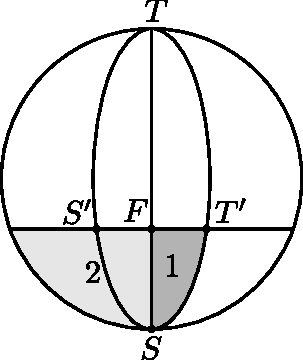
\includegraphics[width=0.6\linewidth]{suvi-joonis-1.pdf}
\end{figure}

Ülejäänud ülesanne taandub geomeetria peale. $FSS'$ ja $FTT'$ pindalad on leitavad vastavate ringi sektorite ning kolmnurkade pindalade kaudu:
\begin{align*}
	T_S &= T_\oplus \frac{S_{FSS'}}{\pi R^2} = T_\oplus \frac{\frac{\varphi}{\ang{360}}\pi R^2 - \frac 12|OF||OS'|\sin\varphi}{\pi R^2}.\\
	&= T_\oplus \left(\frac{\varphi}{\ang{360}} - \frac{\cos\varphi\sin\varphi}{2\pi}\right),\\
\end{align*}
kus me asendasime $|OS'| = R$ ning $|OF| = |OS'|\cos\angle FOS' = R\cos\varphi$. Sarnaselt,
\[
T_T = T_\oplus \left(\frac{\ang{180} - \varphi}{\ang{360}} + \frac{\cos\varphi\sin\varphi}{2\pi}\right).
\]
$\varphi$ saame avaldada kui $\cos\varphi = |OF| / R = (R - d_S) / R$. Samas, $2R = d_T + d_S$, ehk $d_S = 2R/(1 + k)$ ning 
\[
\cos\varphi = 1 - \frac{2}{1 + k} = \frac{k - 1}{k + 1},
\]
ehk
\[
\varphi = \arccos\frac{k - 1}{k + 1} = \arccos\frac{\sqrt{\num{1.3}} - 1}{\sqrt{\num{1.3}} + 1} = \ang{86.24}.
\]
Niisiis, otsitav aegade vahe on 
\[
\Delta T = T_T - T_S = T_\oplus \left(\frac{1}{2} - \frac{\varphi}{\ang{180}} + \frac{\sin\varphi\cos\varphi}{\pi}\right) = \SI{15.2}{päeva}.
\]
\punktid{12} \autor{Erik Tamre}


\yl{KOONUS}
\osa Vaatleme koonuse pinna tasandis toimivaid jõude. Nööri pinge tasakaalustab alati raskusjõu pinnasihilise komponendi, seega pinnasihilised jõud puuduvad, mistõttu liigub kuulike koonuse pinnalaotusel mööda sirgjoont. Seetõttu on teepikkus pinnalaotusel algasendist kuni suurima lähenemiseni tipule $L=l_0\cos\beta$ ning seega otsitav aeg $t=L/v_0=l_0\cos\beta/v_0$. 

\osa Ilmselt on õhku hüppamise mõttes kõige ohtlikum koonilist pinda mööda liikuva kuulikese trajektoori kõrgeim punkt, mille kaugus tipust on $l_0\sin\beta$. Kuivõrd tegemist on kõrgeima punktiga, siis on trajektoori puutujatasand seal horisontaalne ning trajektoori kõverusraadius võrdne antud punkti kaugusega koonuse teljest: $R=l_0\sin\beta\cos\alpha$. Seega on kuulikese kesktõmbekiirendus $a=v_0^2/R$ suunatud horisontaalselt telje suunas. Piirjuhul on selle kiirenduse pinnanormaali sihiline komponent $v_0^2\sin\alpha/R$ võrdne vastava raskuskiirenduse komponendiga $g\cos\alpha$. Seega saame tingimuseks $v_0^2\tan\alpha\le gl_0\sin\beta\cos\alpha$, st $$v_0^2\le \frac{3}{2}gl_0\sin\beta.$$
\punktid{14} \autor{Jaan Kalda}


\end{document}